% !TEX root = ../main.tex
%************************************************
\chapter{Wikipedia as a Data Source for Role Analysis}
\label{app:wikipedia}
%************************************************

\noindent\textit{This appendix outlines preliminary work on leveraging Wikipedia and Wikidata as complementary data sources for understanding organizational role performance. While this analysis extends beyond the scope of the main dissertation, it demonstrates the potential of collaborative knowledge platforms for triangulating findings about how cities and organizations enact climate governance roles. The infrastructure developed here---including automated collection pipelines and analytical frameworks---provides a foundation for future research.}

\bigskip

\section{Rationale and Research Potential}

Wikipedia represents a unique data source for organizational research. Unlike official communications that organizations carefully craft, Wikipedia articles emerge from collaborative editing by diverse contributors, reflecting how organizations are \emph{perceived} and \emph{understood} by external observers. This distinction is theoretically significant for role analysis: while organizational websites and press releases reveal how actors \emph{claim} roles, Wikipedia content illuminates how those roles are \emph{recognized} and \emph{legitimated} by broader publics.

For climate governance specifically, Wikipedia offers several advantages:

\begin{description}
    \item[Temporal depth] Article revision histories enable longitudinal analysis of how organizational representations evolve alongside policy developments and institutional changes.
    \item[Cross-linguistic comparison] Articles in multiple language editions reveal how organizations are framed differently across national and cultural contexts.
    \item[Structured metadata] Wikidata provides machine-readable attributes (founding dates, headquarters, organizational types) that enable systematic comparison.
    \item[Network structure] Internal links between articles map perceived relationships between actors, potentially revealing role constellations.
\end{description}

\section{Data Collection Pipeline}

We developed an automated pipeline for collecting Wikipedia and Wikidata content on entities relevant to the dissertation's empirical focus.

The pipeline follows a straightforward flow: entity lists (NetZeroCities, KIC partners) feed into parallel Wikidata SPARQL queries and Wikipedia API calls. Results are processed into text corpora and feature matrices for role analysis.

\begin{center}
\textbf{Pipeline Overview}

\smallskip
\fbox{Entity Lists} $\rightarrow$ \fbox{Wikidata SPARQL} $\rightarrow$ \fbox{Structured Metadata}

\fbox{Entity Lists} $\rightarrow$ \fbox{Wikipedia API} $\rightarrow$ \fbox{Article Content}

$\downarrow$

\fbox{Data Processing} $\rightarrow$ \fbox{Text Corpus} + \fbox{Features} $\rightarrow$ \fbox{Role Analysis}
\end{center}

\subsection{Wikidata Collection}

Wikidata queries retrieve structured attributes for each entity using SPARQL. For cities, key properties include:

\begin{itemize}
    \item Population time series (P1082)
    \item Geographic coordinates (P625)
    \item Administrative classification (P31)
    \item Climate initiative memberships (P463)
    \item Current mayor/leader (P6)
\end{itemize}

For organizations (EIT KIC partners), we collect:

\begin{itemize}
    \item Organization type (P31)
    \item Founding date (P571)
    \item Headquarters location (P159)
    \item Official website (P856)
    \item Member/partner relationships (P463)
\end{itemize}

\subsection{Wikipedia Article Collection}

The Wikipedia API retrieves full article content including:

\begin{itemize}
    \item Article text (plain and sectioned)
    \item Summary/lead paragraph
    \item Category memberships
    \item Internal wiki-links
    \item Cross-language article links
\end{itemize}

Collection results for the dissertation's focal entities:

\begin{center}
\begin{tabular}{lrrr}
\toprule
\textbf{Entity Type} & \textbf{Total} & \textbf{Articles Found} & \textbf{Coverage} \\
\midrule
NetZeroCities (cities) & 111 & 111 & 100\% \\
EIT KIC Partners (orgs) & 132 & 107 & 81\% \\
\midrule
\textbf{Total} & 243 & 218 & 90\% \\
\bottomrule
\end{tabular}
\end{center}

\section{Information Extraction Pipeline}
\label{sec:wikipedia-pipeline}

Beyond collection, the \texttt{rolebox-wikipedia} module implements a full NLP pipeline for extracting structured information from Wikipedia articles. The pipeline combines multiple extraction techniques:

\begin{description}
    \item[Named Entity Recognition (NER)] Using spaCy's \texttt{en\_core\_web\_sm} model to identify organizations, people, locations, and other named entities mentioned in articles.
    \item[Topic Modeling] BERTopic with sentence transformers discovers latent thematic clusters across the corpus.
    \item[Structured Extraction] NuExtract 1.5, a small language model fine-tuned for template-based extraction, identifies organizational attributes, partnerships, and relationships.
    \item[Entity Linking] Fuzzy matching against known registries plus Wikidata API queries resolve entity mentions to canonical identifiers.
    \item[Powell Triangle Scoring] Keyword-based classification positions each entity on the knowledge triangle (associational, scientific, managerial).
\end{description}

\subsection{Pipeline Results}

Processing results for the dissertation's focal entities:

\begin{center}
\begin{tabular}{lrr}
\toprule
\textbf{Metric} & \textbf{Organizations} & \textbf{Cities} \\
\midrule
Documents processed & 108 & 111 \\
NER entity mentions & 53,835 & 118,939 \\
Topics discovered & 5 & 7 \\
Triangle scores computed & 108 & 111 \\
\bottomrule
\end{tabular}
\end{center}

\subsection{Topic Modeling Results}

BERTopic identified distinct thematic clusters within each corpus. For organizations, the dominant topics reflect institutional types (universities, companies) and sectoral focus areas:

\begin{center}
\small
\begin{tabular}{clr}
\toprule
\textbf{Topic} & \textbf{Representative Keywords} & \textbf{Documents} \\
\midrule
1 & university, research, students & 42 \\
2 & university, college, institute & 28 \\
3 & company, industry, technology & 19 \\
4 & software, digital, innovation & 11 \\
0 & (outlier topic) & 8 \\
\bottomrule
\end{tabular}
\end{center}

For cities, topics capture geographic clustering and urban characteristics:

\begin{center}
\small
\begin{tabular}{clr}
\toprule
\textbf{Topic} & \textbf{Representative Keywords} & \textbf{Documents} \\
\midrule
0 & city, amsterdam, munich & 35 \\
2 & city, italy, milan & 22 \\
3 & city, helsinki, stockholm & 18 \\
4 & city, warsaw, vilnius & 16 \\
\bottomrule
\end{tabular}
\end{center}

\subsection{Powell Triangle Classifications}

The keyword-based scoring positions entities on the knowledge triangle. Results show clear differentiation:

\begin{center}
\begin{tabular}{lrr}
\toprule
\textbf{Classification} & \textbf{Organizations} & \textbf{Cities} \\
\midrule
Dominant Scientific & 61 (56\%) & 24 (22\%) \\
Dominant Managerial & 25 (23\%) & 6 (5\%) \\
Dominant Associational & 5 (5\%) & 10 (9\%) \\
Balanced & 10 (9\%) & 31 (28\%) \\
Mixed & 7 (6\%) & 40 (36\%) \\
\bottomrule
\end{tabular}
\end{center}

Organizations---predominantly universities and research institutes---cluster heavily in the scientific pole (56\%). Cities show more balanced distributions, with the majority classified as ``mixed'' or ``balanced,'' reflecting the multifaceted nature of urban governance that spans community engagement (associational), technical expertise (scientific), and administrative capacity (managerial).

\subsection{Multilingual Capabilities}

The NuExtract 1.5 model supports six European languages (English, French, German, Spanish, Portuguese, Italian), enabling future extension to non-English Wikipedia articles. This multilingual capability is particularly relevant for the EIT ecosystem, which spans organizations across Europe with varying linguistic contexts.

\section{Analytical Possibilities}

The collected Wikipedia data enables several analytical approaches relevant to understanding organizational roles in climate governance. We outline three promising directions below.

\subsection{Role Recognition Through Content Analysis}

Wikipedia article content reveals how external observers characterize organizations. By analyzing the vocabulary, themes, and framings used to describe cities and KIC partners, researchers can assess:

\begin{kaobox}[title=Content Analysis Opportunities]
\begin{itemize}[leftmargin=*]
    \item \textbf{Role vocabulary:} Which role-related terms (innovator, leader, pioneer, partner) appear in organizational descriptions?
    \item \textbf{Domain positioning:} How are organizations situated within thematic fields (climate, energy, urban, technology)?
    \item \textbf{Achievement framing:} What accomplishments and credentials are highlighted?
    \item \textbf{Relationship mapping:} Which other actors are mentioned alongside the focal organization?
\end{itemize}
\end{kaobox}

\subsection{Temporal Evolution of Role Representations}

Wikipedia's revision history API enables longitudinal analysis of how organizational representations change over time. This is particularly valuable for studying:

\begin{itemize}
    \item How city articles incorporated climate commitments following NetZeroCities selection
    \item Evolution of KIC partner descriptions as the EIT ecosystem matured
    \item Response to major policy events (European Green Deal, Fit for 55)
\end{itemize}

\subsection{Cross-Linguistic Role Framing}

Many cities and organizations have Wikipedia articles in multiple languages. Cross-linguistic comparison can reveal:

\begin{itemize}
    \item National vs. European framings of climate leadership
    \item Local vs. international recognition of organizational roles
    \item Cultural variation in how innovation and sustainability are conceptualized
\end{itemize}

\section{Sample Data and Illustrations}

To illustrate the richness of Wikipedia data, we present examples from the collected corpus.

\subsection{City Article Structure}

Key metrics for selected NetZeroCities Wikipedia articles:

\begin{center}
\small
\begin{tabular}{lrrrr}
\toprule
\textbf{City} & \textbf{Text Length} & \textbf{Sections} & \textbf{Categories} & \textbf{Links} \\
\midrule
Amsterdam & 156,234 & 42 & 89 & 1,247 \\
Copenhagen & 98,451 & 35 & 67 & 892 \\
Barcelona & 187,892 & 48 & 112 & 1,456 \\
Stockholm & 112,567 & 38 & 78 & 1,034 \\
Helsinki & 89,234 & 31 & 54 & 756 \\
\bottomrule
\end{tabular}
\end{center}

\subsection{Organization Description Patterns}

Excerpts from EIT KIC partner articles reveal characteristic patterns in how organizations are described. The following examples illustrate different role framings:

\begin{kaobox}[title=Example: Research Institution Role]
``\textit{ETH Zurich is a public research university in the city of Zurich, Switzerland. Founded in 1854, it is one of the world's leading universities for technology and natural sciences, particularly in the fields of engineering, mathematics, and physics.}''
\end{kaobox}

\begin{kaobox}[title=Example: Industry Partner Role]
``\textit{Siemens AG is a German multinational conglomerate corporation and the largest industrial manufacturing company in Europe. The principal divisions of the company are Industry, Energy, Healthcare, and Infrastructure \& Cities.}''
\end{kaobox}

\section{Technical Implementation}

The collection pipeline is implemented in Python and available in the \texttt{rolebox-wikipedia} repository. Key components include:

\begin{lstlisting}[language=Python, caption={Wikidata SPARQL query for city attributes}, label={lst:sparql-city}]
SELECT ?city ?cityLabel ?population ?coordinates
WHERE {
    BIND(wd:Q727 AS ?city)  # Amsterdam
    OPTIONAL { ?city wdt:P1082 ?population. }
    OPTIONAL { ?city wdt:P625 ?coordinates. }
    SERVICE wikibase:label {
        bd:serviceParam wikibase:language "en".
    }
}
\end{lstlisting}

\begin{lstlisting}[language=Python, caption={Wikipedia article content retrieval}, label={lst:wikipedia-api}]
import wikipediaapi

wiki = wikipediaapi.Wikipedia(
    user_agent='RoleboxWikipedia/1.0',
    language='en'
)

page = wiki.page("Amsterdam")
print(page.summary)  # Lead paragraph
print(page.text)     # Full article text
print(page.sections) # Section structure
\end{lstlisting}

\begin{lstlisting}[language=Python, caption={Running the full NLP extraction pipeline}, label={lst:pipeline}]
from rolebox_wikipedia import WikipediaPipeline, PipelineConfig

config = PipelineConfig(
    enable_nuextract=True,          # Structured extraction
    nuextract_model="sroecker/nuextract-tiny-v1.5",
    enable_topic_modeling=True,     # BERTopic
    enable_triangle_scoring=True,   # Powell framework
    enable_entity_linking=True,     # Wikidata linking
)

pipeline = WikipediaPipeline(config=config)
results = pipeline.run(
    corpus_path="data/orgs_text_corpus.json",
    orgs_registry_path="data/orgs_wikidata.csv",
)

# Access results
print(f"Entities: {results.processing_stats['ner_entities']}")
print(f"Topics: {results.processing_stats['num_topics']}")
results.save("pipeline_results.json")
\end{lstlisting}

\section{Knowledge Graph Extraction}
\label{sec:wikipedia-kggen}

Beyond topic modeling and structured extraction, we employed \textbf{kg-gen}, an LLM-based knowledge graph extraction library, to identify entities and relations directly from Wikipedia article text. Using Llama 3.2 via Ollama, the pipeline processes each article and extracts subject-predicate-object triples.

\subsection{Extraction Results}

Processing the 108 EIT partner organization Wikipedia articles yielded:

\begin{center}
\begin{tabular}{lr}
\toprule
\textbf{Metric} & \textbf{Value} \\
\midrule
Documents processed & 106 \\
Unique entities extracted & 1,311 \\
Unique relations & 1,330 \\
Edge types (predicates) & 734 \\
\bottomrule
\end{tabular}
\end{center}

The extracted knowledge graph captures institutional relationships, geographic associations, founding dates, organizational types, and research domains. Entity types include organizations (universities, companies), locations (cities, countries), persons (founders, notable alumni), and concepts (research fields, technologies).

\subsection{Visualization}

Figure~\ref{fig:kg-wikipedia} shows a network visualization of the aggregated knowledge graph. Organizations cluster around shared predicates such as ``located in,'' ``founded in,'' and ``member of.'' Central hub entities like ``Europe,'' ``university,'' and ``research'' connect disparate organizational nodes.

\begin{center}
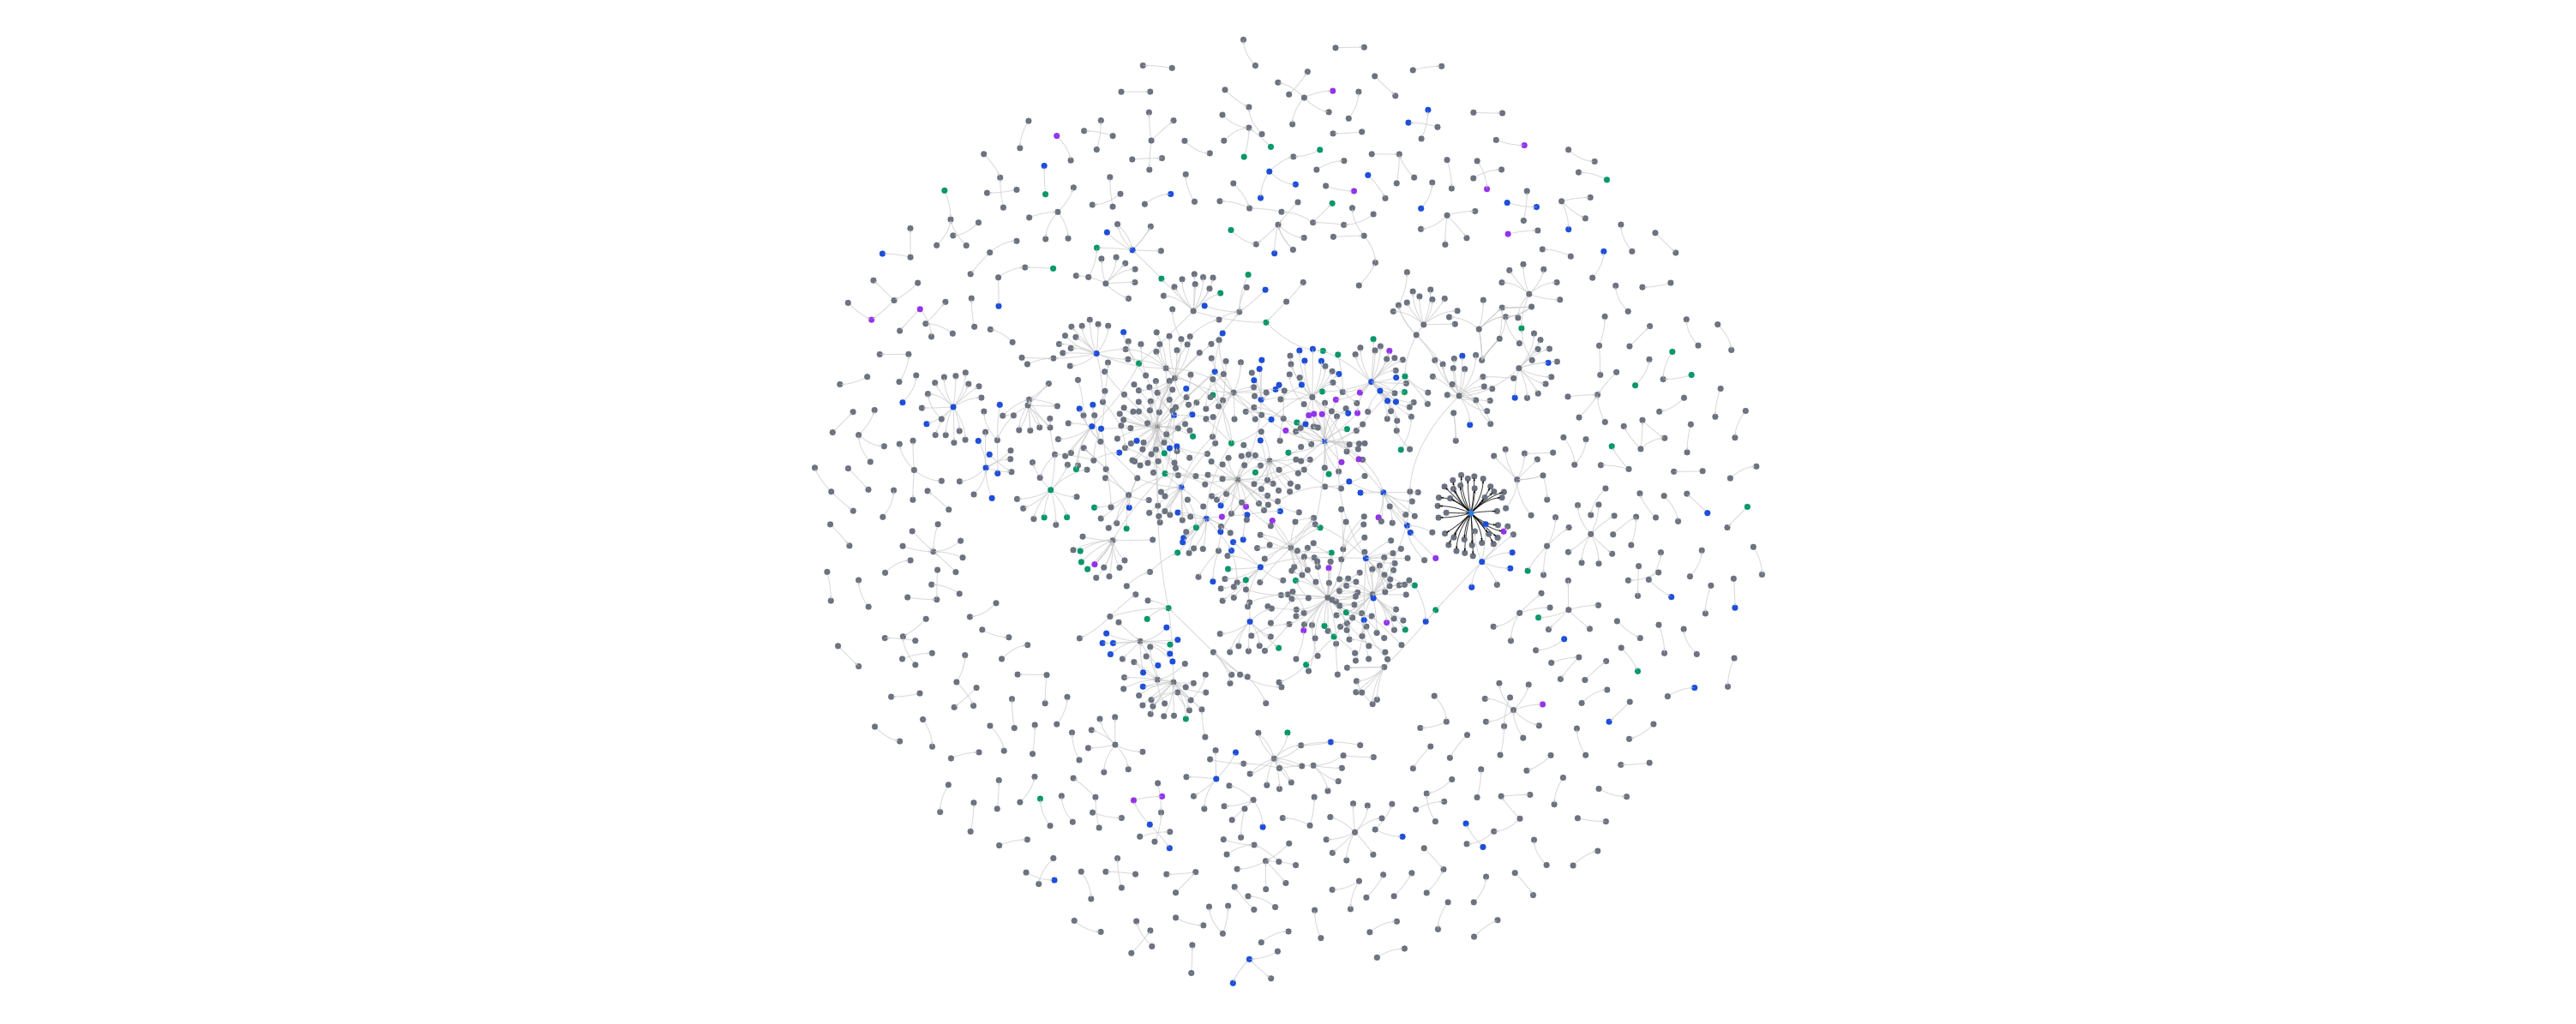
\includegraphics[width=0.85\textwidth]{figures/kg_wikipedia_orgs.png}
\captionof{figure}{Knowledge graph extracted from 106 EIT partner Wikipedia articles using kg-gen with Llama 3.2. Node colors: blue (organization), green (location), purple (person), gray (concept).}
\label{fig:kg-wikipedia}
\end{center}

The interactive version of this visualization is available in the \texttt{rolebox-wikipedia} repository at \texttt{ui/rolebox\_wikipedia\_eit-kg.html}.

\section{Limitations and Future Work}

This preliminary analysis has several limitations that future research should address:

\begin{enumerate}
    \item \textbf{Snapshot data:} Current collection captures a single point in time; longitudinal tracking would require periodic re-collection or revision history analysis.

    \item \textbf{English-only:} Articles were collected only from English Wikipedia; multi-language analysis requires additional collection and translation/alignment procedures.

    \item \textbf{QID accuracy:} Some Wikidata entity identifiers returned incorrect matches, requiring manual verification for production use.

    \item \textbf{Coverage gaps:} Not all organizations have Wikipedia articles, potentially introducing selection bias toward more prominent actors.
\end{enumerate}

Future work could extend this foundation in several directions:

\begin{kaobox}[title=Research Extensions]
\begin{description}[leftmargin=*]
    \item[Revision history analysis] Track how organizational representations evolve over time in response to policy developments.
    \item[Editor network analysis] Map the community of contributors editing climate governance articles.
    \item[Cross-platform comparison] Compare Wikipedia representations with organizational self-presentations.
    \item[Multilingual role framing] Analyze how roles are framed differently across language editions.
    \item[Link network analysis] Use wiki-links to map perceived relationships between actors.
\end{description}
\end{kaobox}

\section{Conclusion}

Wikipedia and Wikidata offer valuable complementary data sources for studying organizational role performance in climate governance. While the analysis presented here is preliminary, the collection infrastructure and analytical frameworks developed provide a foundation for future research. The key insight is that Wikipedia captures \emph{external recognition} of organizational roles---how actors are perceived and categorized by diverse observers---complementing the \emph{internal claims} revealed through organizational communications analysis.

The intersection of collaborative knowledge production and institutional role theory presents fertile ground for future scholarship. As Wikipedia continues to grow and evolve, its potential as a source for understanding how organizations are situated within complex governance fields will only increase.
